%\begin{figure*}
%        \includegraphics[width=\textwidth,height=5cm]{tensorflow-tika-integration}
%        \caption{Tika and Tensorflow Integration}
%        \label{fig:tf-tika-integration}
%\end{figure*}

\section{INTEGRATION} \label{sec:integration}
To integrate Tika and Tensorflow, we extended Tika's \texttt{Recogniser} interface which was introduced as part of our work in integrating named entity recognition (NER) toolkits ddescribed in the prior section. Our new interface was called \texttt{ObjectRecogniser}. The goal of \texttt{ObjectRecogniser} is to facilitate multiple implementations that extend beyond Tensorflow and that may include other future deep learning and other recognition frameworks. The main component of the interface contract is a function that accepts image data and returns a list of \texttt{RecognisedObject}s.

For our initial implementation of \texttt{ObjectRecogniser} we created a python based command line (CLI) tool as an entry point to Tensorflow's image recognition network. This tool inspected the environment for its requirements which included the Tensorflow command line tool, and when its requirements were not met it failed and reported the failure. Apache Tika executed in the JVM process where -- as on every invocation of CLI tool -- a new native process was created and destroyed. Tika passed image path as a command line argument to the tool as shown in Figure \ref{fig:tf-tika-integration} (a). The tool parsed the arguments, then passed the content to the Tensorflow network and reported the results by printing it to standard output. Tika parser then read the result from its output stream. We did not extend Tensorflow's existing ImageNet/Inception model training and simply used it out of the box already configured in the Tensorflow python program.

The Java Native Interface (JNI) is vendors' recommended way of integrating native code libraries to Java frameworks\cite{gordon1998essential}. JNI acts as glue between bytecode instructions that run within the Java Virtual Machine (JVM) and the native code instructions that run directly on the CPU. Theoretically, this is the best way of merging the JVM world with the native code. At runtime, the bytecode of Tika (caller) and native code of tensorflow (callee) runs within a single process from the operating system's perspective as shown in Figure \ref{fig:tf-tika-integration} (b).

The developers of Tensorflow framework recommended using gRPC based integration for the production systems\cite{goog-tfserve}. gRPC is a client-server based architecture in which caller acts as an RPC client and callee serves as a server in a different address space. Unlike traditional RPC frameworks, gRPC is a high-performance, high-CPU, and bandwidth efficient transport on top of HTTP/2 that supports full duplex streaming\cite{about-grpc}. In our case, we embedded gRPC client in Tika JVM and exported Tensorflow image recognition capabilities as remote procedures via gRPC service. We used Tensorflow Serving, a gRPC server implemented in C++, and also created a docker container to host it.  Collecting the needed libraries to build the gRPC interface proved to be a non-trivial effort, and rather than require users of our Tika and Tensorflow integration to install these libraries, we also investigated building a Representation State Transfer (REST) interface \cite{Fielding:2000:ASD:932295}.

REST is a client-server architecture paradigm for connecting heterogeneous systems without the need of states \cite[Chapter~5]{Fielding:2000:ASD:932295}. The REST application programming interfaces (API) is powered by the HyperText Transfer Protocol (HTTP) which abstracts the complexities of Transmission Control Protocol.
We created REST API for Tensorflow image recognition using python Flask. The Flask based HTTP service registered a TCP port and offered HTTP API endpoints as shown in Figure \ref{fig:tf-tika-integration} (d), and the REST interface had the advantage of minimizing client dependencies for using our framework. REST clients are light-weight and have easily installable dependencies across all major programming languages. Our REST API endpoint accepted HTTP POST requests with image data in the request body. This service loaded the Inception v3 \cite{SzegedyVISW15} model during the initialization phase and held the model in memory for reusing it during the future HTTP Requests.

% \begin{figure}[h]
%     \centering
%     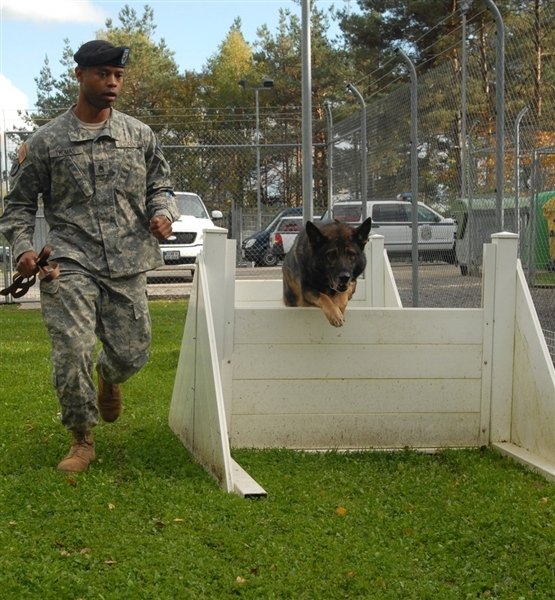
\includegraphics[width=\columnwidth]{military_dog}
%     \caption{Military Person with a German Shepherd Dog \newline Courtesy: Wikimedia Commons}
%     \label{fig:military-dog}
% \end{figure}

% The REST API, upon recognizing the objects in the image \ref{fig:military-dog}, returned the response in the JSON format with the following structure:

% \begin{lstlisting}[language=json, label=code:json-output,
% 	frame=single, xleftmargin=5.0pt, xrightmargin=5.0pt,
%     caption=JSON Response from REST API]
% {
%   "confidence": [ 0.362026, 0.130613],
%   "classnames": [
%     "German shepherd, alsatian",
%     "military uniform"
%   ],
%   "classids": [211, 866 ],
%   "time": {
%     "read": 1,
%     "units": "ms",
%     "classification": 257
%   }
% }
% \end{lstlisting}

On the other side of the system, we implemented the class \texttt{TensorflowRESTRecogniser} which used HTTP Client to communicate with the REST API. This implementation of \texttt{ObjectRecogniser} converted the image data to HTTP POST request with multipart form data and sent it to REST API. It parsed the JSON response to retrieve the object names, IDs and confidence scores. We also created a Docker specification for bootstrapping the Tensorflow image recognition REST API for semi-automated deployment of the system. We created the Docker to provide an easily usable client and server for Tensorflow Tika integration providing all needed dependencies and capabilities for the integration automatically.

%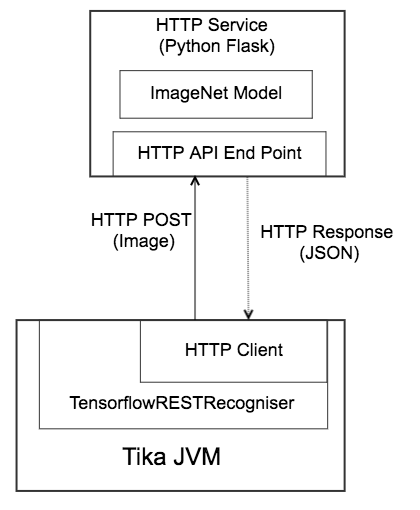
\includegraphics[scale=0.40]{tika-tflow-rest-design}
